\section{Hadoop 1}

\begin{figure}[H]
    \centering
    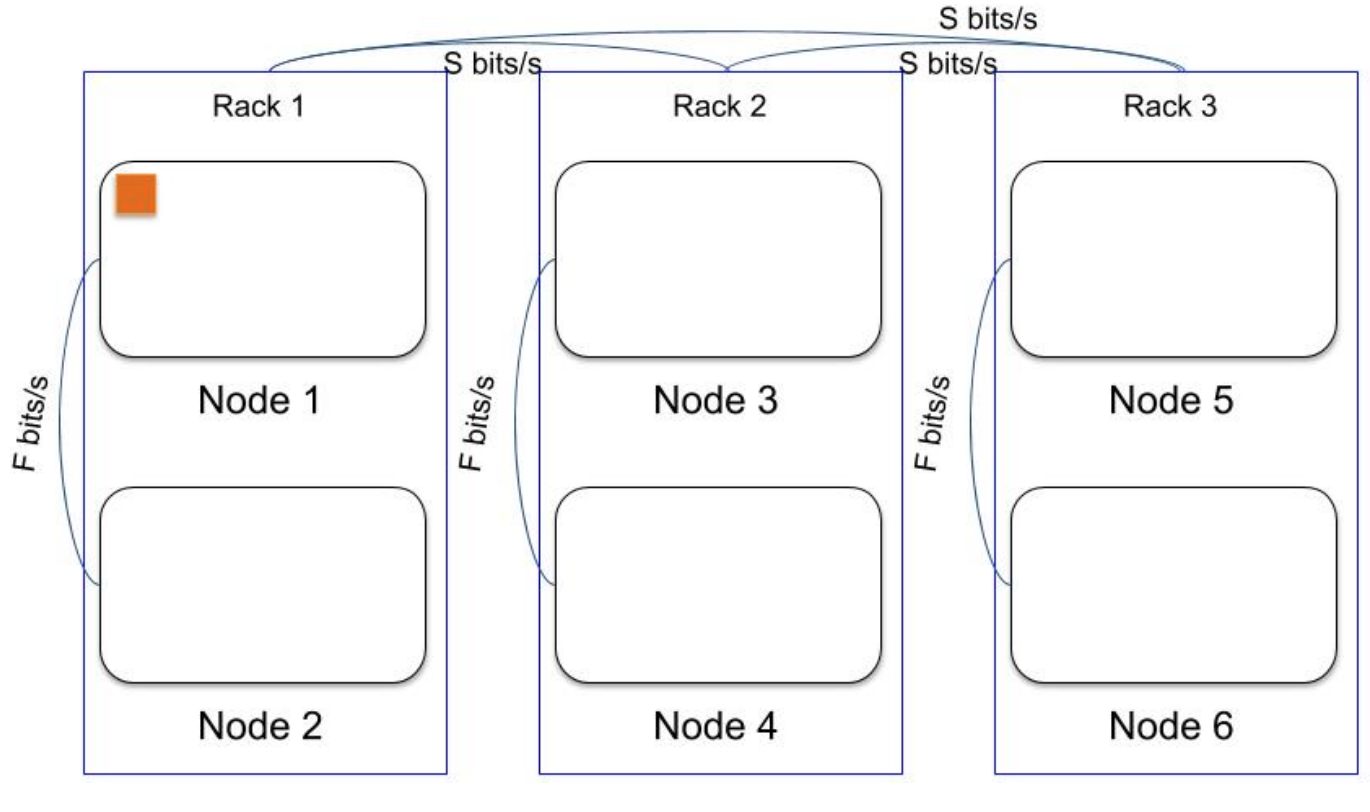
\includegraphics[width=0.7\textwidth]{figures/hadoop1/case.png}
    \caption{Hadoop Case}
    \label{fig:case}
\end{figure}

\textbf{Hadoop Replication Strategy}
\begin{enumerate}
    \item One replica on local node
    \item Second replica on a remote rack
    \item Third replica on same remote rack
    \item Additional replicas are randomly placed
\end{enumerate}

\textbf{Problem}
\begin{itemize}
    \item[\textbf{P1}] How would Hadoop create 3 replicas in total? Write all set of nodes that could be selected\\
    $P = \{3,4\} v \{5,6\}$
    \item[\textbf{P2}] The time $T1$ to replicate D bits from Node 1 using the sets from P1\\
    $T1(D)=\frac{S}{D}+\frac{F}{D}$ 
    \item[\textbf{P3}] The time $T2$ to replicate to two racks take Node 3 and Node 5 and the gain factor $G=\frac{T2}{T1}$\\
    $T2(D)=2\cdot\frac{S}{D}$ \\
    $G=\frac{T2}{T1}=2\cdot\frac{\frac{S}{D}}{\frac{S}{D}+\frac{F}{D}}=\frac{2S}{F+S}$
    \item[\textbf{P4}] Compute average time $T3$ using 4 replicas and $T4$ using 5 replicas\\\\
    The first three replications would follow the same procedure as $T1$, the next replication would be selected at random (between node 2, 5 or 6, e.g. on a other rack)
    The first 3 replicas will follow a consistent pattern. The following replicas are selected at random. \\
    $T3(D)=2\cdot\frac{S}{D}+\frac{F}{D}$ \\\\
    If the fourth node would be 5 or 6, and the fifth node would be the other one, the last replication would be intra-rack\\
    $T4(D)_1=2\cdot\frac{S}{D}+2\cdot\frac{F}{D}$\\
    else the last replication would be inter-rack\\
    $T4(D)_2=3\cdot\frac{S}{D}+\frac{F}{D}$ \\
    Average: $T4(D)_1$ applies to two combination, and $T4(D)_2$ to the other four.\\
    $T4(D)_{avg} = \frac{1}{3} \cdot T4(D)_1 + \frac{2}{3} \cdot T4(D)_2 = 2\frac{2}{3}\cdot\frac{S}{D} + 1\frac{1}{3}\cdot\frac{F}{D}$
\end{itemize}